
% ----------------------------------------------------------------------
%  Set the document class
% ----------------------------------------------------------------------
\documentclass[11pt,a4paper,twoside]{article}

% ----------------------------------------------------------------------
% Define external packages, language, margins, fonts and new commands
% ----------------------------------------------------------------------
%\input{preamble} 
\usepackage[utf8]{inputenc}   % <<<<< Linux
\usepackage[english]{babel} % <<<<< English
\usepackage{notoccite}
\usepackage[skip=0.5\baselineskip]{caption}
\hyphenation{GTKWave}
\usepackage{listings}
\usepackage[all]{nowidow}
\usepackage{tabularx}
\usepackage{amsmath}
\usepackage{float}

%blind text
\usepackage{lipsum}

\usepackage{graphicx}
\graphicspath{ {./} {../../figlib/} }
\def\FontLn{% 16 pt normal
  \usefont{T1}{phv}{m}{n}\fontsize{16pt}{16pt}\selectfont}
\def\FontLb{% 16 pt bold
  \usefont{T1}{phv}{b}{n}\fontsize{16pt}{16pt}\selectfont}
\def\FontMn{% 14 pt normal
  \usefont{T1}{phv}{m}{n}\fontsize{14pt}{14pt}\selectfont}
\def\FontMb{% 14 pt bold
  \usefont{T1}{phv}{b}{n}\fontsize{14pt}{14pt}\selectfont}
\def\FontSn{% 12 pt normal
  \usefont{T1}{phv}{m}{n}\fontsize{12pt}{12pt}\selectfont}

% Use Arial font as default
%
\renewcommand{\rmdefault}{phv}
\renewcommand{\sfdefault}{phv}
\usepackage{geometry}	
\geometry{verbose,tmargin=2.5cm,bmargin=2.5cm,lmargin=2.5cm,rmargin=2.5cm}

%\usepackage{setspace}
%\renewcommand{\baselinestretch}{1.5}

\usepackage[pdftex]{hyperref} % enhance documents that are to be
                              % output as HTML and PDF
\hypersetup{colorlinks,       % color text of links and anchors,
                              % eliminates borders around links
%            linkcolor=red,    % color for normal internal links
            linkcolor=black,  % color for normal internal links
            anchorcolor=black,% color for anchor text
%            citecolor=green,  % color for bibliographical citations
            citecolor=black,  % color for bibliographical citations
%            filecolor=magenta,% color for URLs which open local files
            filecolor=black,  % color for URLs which open local files
%            menucolor=red,    % color for Acrobat menu items
            menucolor=black,  % color for Acrobat menu items
%            pagecolor=red,    % color for links to other pages
            pagecolor=black,  % color for links to other pages
%            urlcolor=cyan,    % color for linked URLs
            urlcolor=black,   % color for linked URLs
	          bookmarks=true,         % create PDF bookmarks
	          bookmarksopen=false,    % don't expand bookmarks
	          bookmarksnumbered=true, % number bookmarks
	          pdftitle={report},
            pdfauthor={Andre C. Marta},
%            pdfsubject={Thesis Title},
%            pdfkeywords={Thesis Keywords},
            pdfstartview=FitV,
            pdfdisplaydoctitle=true}

\usepackage[numbers,sort&compress]{natbib} % <<<<< References in numbered list [1],[2],...
\usepackage{subcaption} 
\usepackage{mdframed}

%%%%%%%%%%%%%%%%%%%%%%%%%%%%%%%%%%%%%%%%%%%%%%%%%%%%%%%%%%%%%%%%%%%%%%%%
%     Begin Document                                                   %
%%%%%%%%%%%%%%%%%%%%%%%%%%%%%%%%%%%%%%%%%%%%%%%%%%%%%%%%%%%%%%%%%%%%%%%%


\begin{document}

% Set plain page style (no headers, footer with centered page number)
\pagestyle{plain}

% Set roman numbering (i,ii,...) before the start of chapters
%\pagenumbering{roman}

% ----------------------------------------------------------------------
%  Cover page
% ----------------------------------------------------------------------
%%%%%%%%%%%%%%%%%%%%%%%%%%%%%%%%%%%%%%%%%%%%%%%%%%%%%%%%%%%%%%%%%%%%%%%%
%                                                                      %
%     File: Thesis_FrontCover.tex                                      %
%     Tex Master: Thesis.tex                                           %
%                                                                      %
%     Author: Andre C. Marta                                           %
%     Last modified :  2 Jul 2015                                      %
%                                                                      %
%%%%%%%%%%%%%%%%%%%%%%%%%%%%%%%%%%%%%%%%%%%%%%%%%%%%%%%%%%%%%%%%%%%%%%%%

\thispagestyle {empty}


% IST Logo - Signature A
% parameters: bb=llx lly urx ury (bounding box), width=h_length, height=v_length, angle=angle, scale=factor, clip=true/false, draft=true/false. 
\includegraphics[bb=9.5cm 11cm 0cm 0cm,scale=0.29]{IST_A_CMYK_POS}

\begin{center}
%
% Figure (Image or plot)
\vspace{1.0cm}
% height = 50 mm
%\includegraphics[height=50mm]{Figures/Airbus_A350.jpg}

% Title, author and degree
\vspace{1cm}
{\FontLb Circuit Theory and Electronics Fundamentals} \\ % <<<<< EDIT TITLE
\vspace{1cm}
{\FontSn Aerospace Engineering, Técnico, University of Lisbon} \\ % <<<<< EDIT COURSE
\vspace{1cm}
{\FontSn 4\textsuperscript{th} Laboratory Report} \\
\vspace{1cm}
{\FontSn João Martins 95806} \\
{\FontSn Gonçalo Martins 95793}\\
{\FontSn António Lopes 95771}\\
\vspace{1cm}
{\FontSn May 23, 2021} \\ % <<<<< EDIT DATE (corresponds to date of oral examination)
%
\end{center}










% ----------------------------------------------------------------------
% Dedication page (optional)
% ----------------------------------------------------------------------
%\input{dedication} 
%\cleardoublepage

% ----------------------------------------------------------------------
%  Acknowledgments (optional)
% ----------------------------------------------------------------------
%\input{acknowledgements}
%\cleardoublepage

% ----------------------------------------------------------------------
%  Abstract (both in English and Portuguese)
% ----------------------------------------------------------------------
%\input{resumo} 
%\cleardoublepage

%\input{abstract} 

% ----------------------------------------------------------------------
%  Table of contents, list of tables, list of figures and nomenclature
% ----------------------------------------------------------------------

% Table of contents
%
\tableofcontents

% List of tables
%\addcontentsline{toc}{section}{\listtablename}
%\listoftables
%\cleardoublepage 

% List of figures
%\addcontentsline{toc}{section}{\listfigurename}
%\listoffigures
%\cleardoublepage 

% Set arabic numbering (1,2,...) after preface
%
%\setcounter{page}{1}
%\pagenumbering{arabic}

% ----------------------------------------------------------------------
%  Body
% ----------------------------------------------------------------------
\newpage
\section{Introduction}
\label{sec:introduction}

% state the learning objective 
The objective of this laboratory assignment is to study a circuit containing a
sinusoidal voltage source $V_I$ connected to a resistor $R$ and a capacitor $C$
in series. The circuit can be seen if Figure~\ref{fig:rc}.

\lipsum[1-1]

In Section~\ref{sec:analysis}, a theoretical analysis of the circuit is
presented. In Section~\ref{sec:simulation}, the circuit is analysed by
simulation, and the results are compared to the theoretical results obtained in
Section~\ref{sec:analysis}. The conclusions of this study are outlined in
Section~\ref{sec:conclusion}.

\begin{figure}[h] \centering
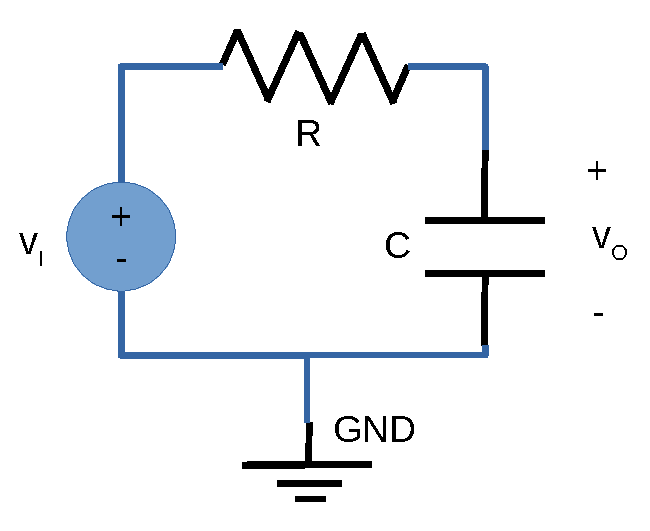
\includegraphics[width=0.4\linewidth]{rc.pdf}
\caption{Voltage driven serial RC circuit.}
\label{fig:rc}
\end{figure}


\newpage
\section{Theoretical Analysis}
\label{sec:theoretical}

\noindent \par In this section, the circuit shown in Figure~\ref{fig:Esquema_teo} is analysed theoretically, considering

\begin{equation}
	v_s(t) = V_s u(-t) + sin(2 \pi ft)u(t)
\end{equation}

with

\begin{equation}
u(t)= \begin{cases} 
	     0, & t<0; \\ 
	     1, & t \geq 0. \\
      \end{cases}
\end{equation}
and

\begin{table}[H]
\centering
\begin{tabularx}{0.8\textwidth} {
  | >{\raggedright\arraybackslash}X
  | >{\raggedleft\arraybackslash}X | }
 \hline
 R1 & 1.006765e+03 Ohm \\ \hline
R2 & 2.033032e+03 Ohm \\ \hline
R3 & 3.033913e+03 Ohm \\ \hline
R4 & 4.003128e+03 Ohm \\ \hline
R5 & 3.131011e+03 Ohm \\ \hline
R6 & 2.093899e+03 Ohm \\ \hline
R7 & 1.017744e+03 Ohm \\ \hline
Vs & 5.223200e+00 V \\ \hline
C & 1.035361e-06 F \\ \hline
Kb & 7.272764e-03 S \\ \hline
Kd & 8.170065e+03 Ohm \\ \hline

\end{tabularx}
\end{table}

\begin{figure}[H] \centering
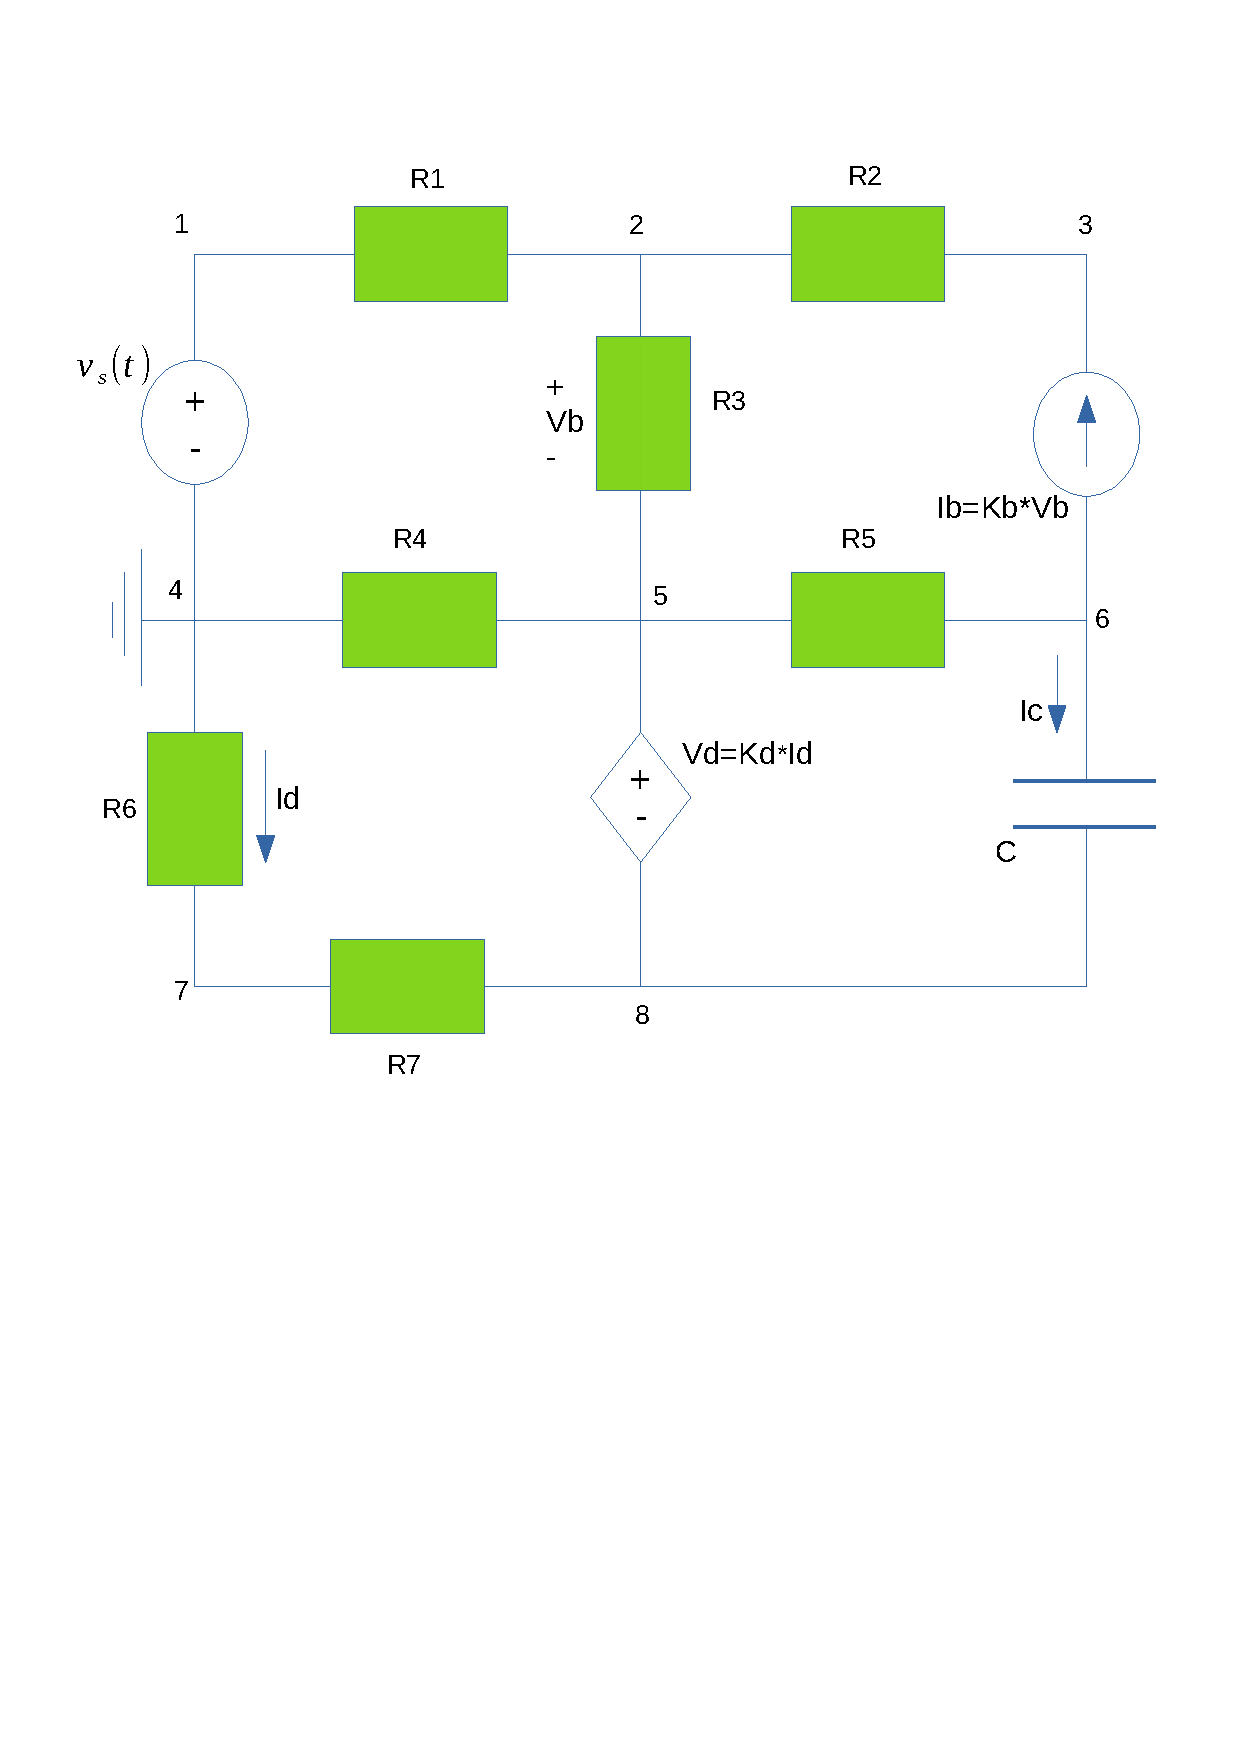
\includegraphics[width=0.8\linewidth]{Esquema_teo.pdf}
\caption{Circuit analysed during the lab assignment}
\label{fig:Esquema_teo}
\end{figure}

\subsection{First point}
\label{ssec:1T}
\noindent \par In the first point, the goal is to perform node analysis for $t<0$, to determine all node voltages.
\par In order to do this we did KCL in each node, considering that all currents were diverging from it, which lead us to the following matrix equation

\begin{equation}
\label{eq:teo1}
	\begin{bmatrix}
	1 & 0 & 0 & 0 & 0 & 0 & 0 & 0 \\ -G1 & G1+G2+G3 & -G2 & 0 & -G3 & 0 & 0 & 0 \\ 0 & -G2-Kb & G2 & 0 & Kb & 0 & 0 & 0 \\ 0 & 0 & 0 & 1 & 0 & 0 & 0 & 0 \\ 0 & 0 & 0 & Kd \cdot G6 & -1 & 0 & -Kd 		\cdot G6 & 1 \\ 0 & Kb & 0 & 0 & -Kb-G5 & G5 & 0 & 0 \\ 0 & 0 & 0 & -G6 & 0 & 0 & G6+G7 & -G7 \\ 0 & -G3 & 0 & -G4-G6 & G3+G4+G5 & -G5 & G6 & 0 \\
	\end{bmatrix}
	\begin{bmatrix}
	V1 \\ V2 \\ V3 \\ V4 \\ V5 \\ V6 \\ V7 \\ V8
	\end{bmatrix}
	=
	\begin{bmatrix}
	Vs \\ 0 \\ 0 \\ 0 \\ 0 \\ 0 \\ 0 \\ 0
	\end{bmatrix}
\end{equation}

\par Solving equation \ref{eq:teo1}, we get the following result

\begin{table}[H]
\centering
\begin{tabularx}{0.8\textwidth} {
  | >{\raggedright\arraybackslash}X
  | >{\raggedleft\arraybackslash}X | }
 \hline
 V1 & 5.223200e+00 V \\ \hline
V2 & 4.960945e+00 V \\ \hline
V3 & 4.406214e+00 V \\ \hline
V4 & 0.000000e+00 V \\ \hline
V5 & 4.998463e+00 V \\ \hline
V6 & 5.852787e+00 V \\ \hline
V7 & -2.069080e+00 V \\ \hline
V8 & -3.074760e+00 V \\ \hline

\end{tabularx}
\end{table}

\par Knowing all node voltages, we can determine Ib, then use Ohm's law in resistors R1 and R6, and finally we can use mesh analysis to determine all branch currents.

\begin{figure}[H] \centering
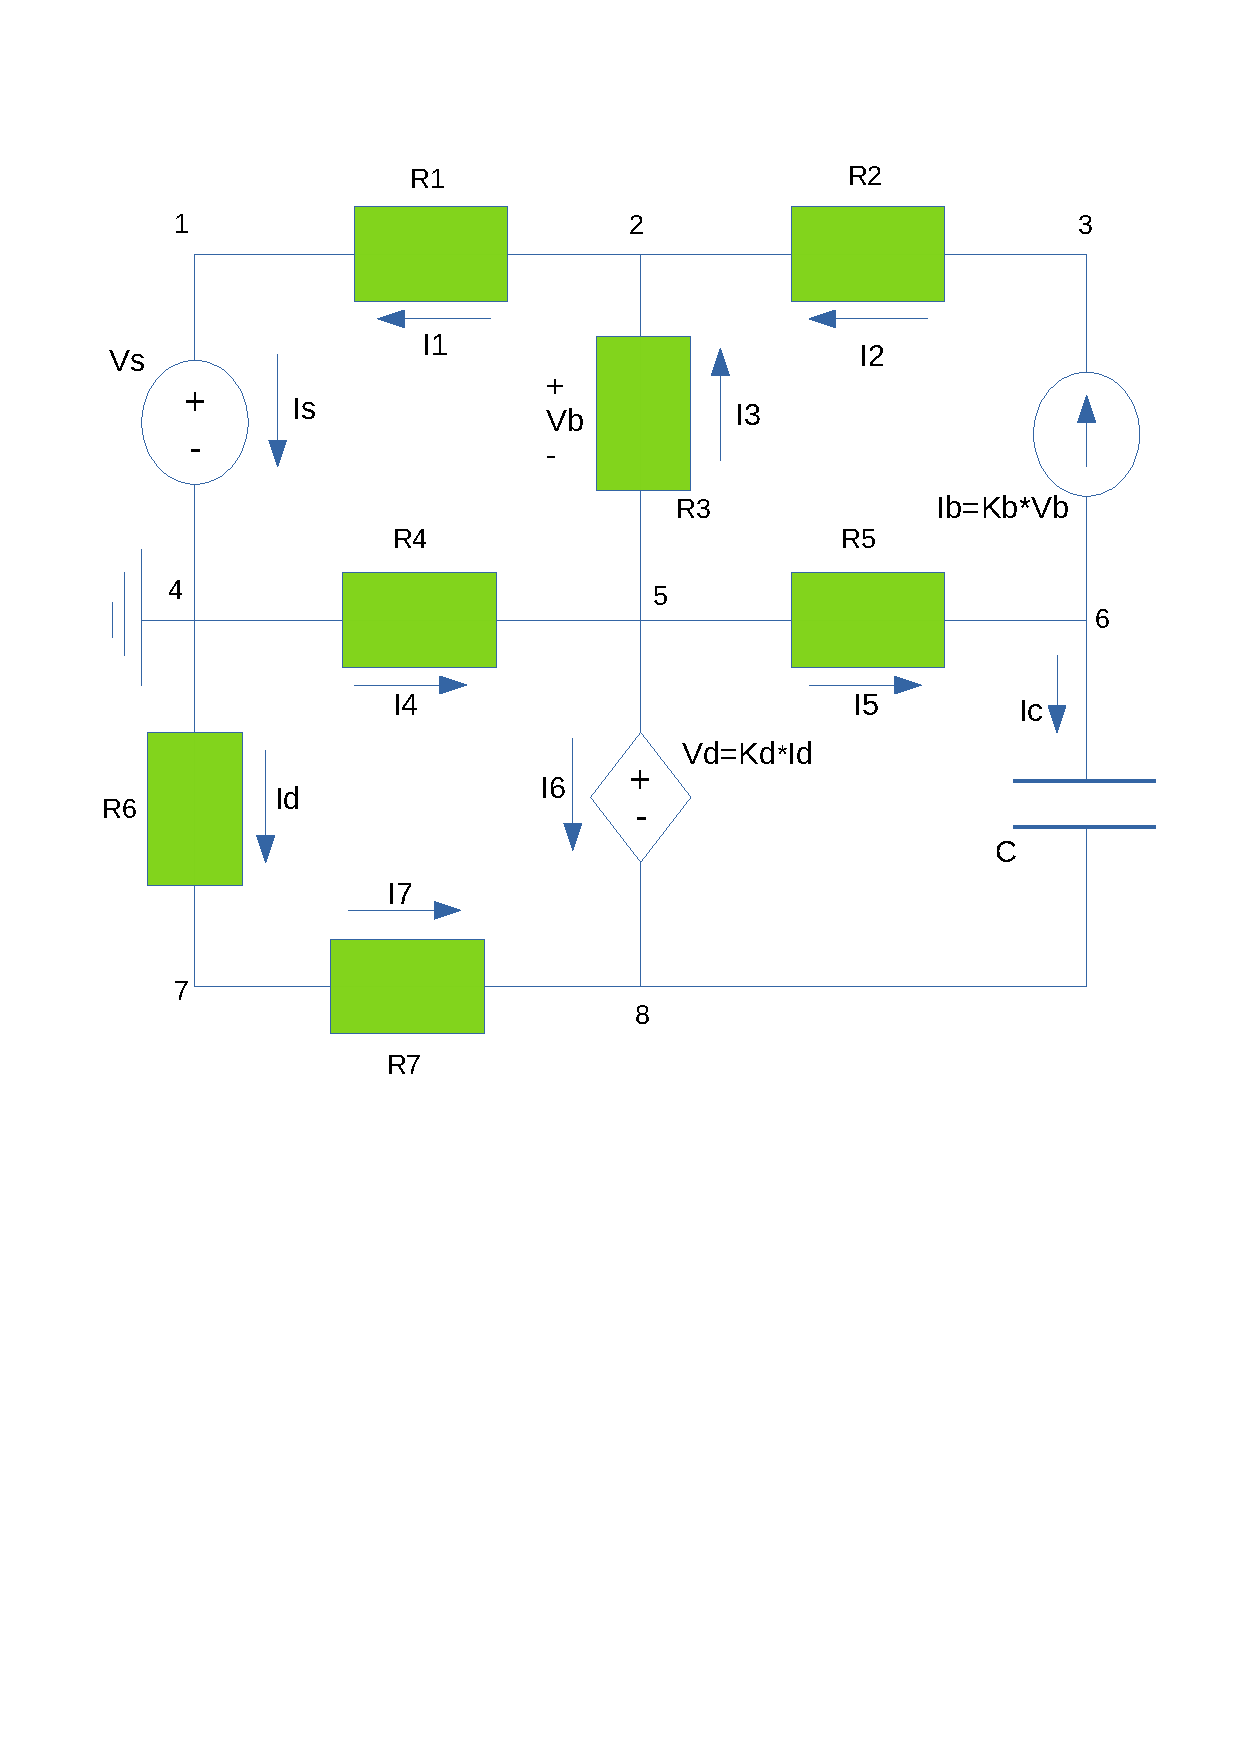
\includegraphics[width=0.8\linewidth]{Esquema1_currents_teo.pdf}
\caption{Current directions considered to determine all branch currents}
\label{fig:Esquema1_currents_teo}
\end{figure}

\par Considering the current directions shown in figure \ref{fig:Esquema1_currents_teo}, we get the following result

\begin{table}[H]
\centering
\begin{tabularx}{0.8\textwidth} {
  | >{\raggedright\arraybackslash}X
  | >{\raggedleft\arraybackslash}X | }
 \hline
 I1 & -2.604926e-04 A \\ \hline
I2 & -2.728588e-04 A \\ \hline
I3 & 1.236617e-05 A \\ \hline
I4 & -1.248639e-03 A \\ \hline
I5 & -2.728588e-04 A \\ \hline
I6 & 9.881466e-04 A \\ \hline
I7 & 9.881466e-04 A \\ \hline
Is & -2.604926e-04 A \\ \hline
Ic & 0.000000e+00 A \\ \hline
Id & 9.881466e-04 A \\ \hline

\end{tabularx}
\end{table}


	



\section{Theoretical Analysis}
\label{sec:theoretical}

\par In this section, the circuit shown in figure \ref{fig:1} is analysed theoretically.
\par Like we said in section \ref{sec:introduction}, both of the stages of the amplifier are going to be analysed in a more detailed way in this section.
\par Let's begin with the gain stage. The gain stage consists of a common emitter amplifier, with a NPN transistor, which allows us to obtain a high input impedance ($Z_{i_1}$), and a high gain $A_V$. However, this type of amplifier has a very high output impedance ($Z_{o_1}$), which causes a degeneration of the signal output. In order to solve this problem, the gain stage is connected to an output stage, which consists of a common collector amplifier, whith a PNP transistor. This stage has a gain a little bit lower than 1, but still very close to 1, and a very high input impedance ($Z_{o_2}$), which preserve the high gain of the previous stage. In addition, this circuit has a very low output impedance ($Z_{o_2}$), which means that almost all the gain is going to be delivered to the speaker.

\subsection{First Point}

\par Our theoretical analysis starts by computing the operating point, using the theoretical DC model studied. In order to do this, we harnessed the mesh method provided in the Octave script to which we added the new components.
\par The values of currents are presented in table \ref{tab:currents}, as well as the values of $V_{CE}$ and $V_{BE}$, and $V_{EC}$ and $V_{EB}$, respectively for the NPN and the PNP transistors, in order to prove that they're working in the forward active region ($V_{CE} > V_{BEON}$ and $V_{EC} > V_{EBON}$).


\vspace{5mm}
\begin{table}[H]
	\centering
	\begin{tabularx}{0.9\textwidth} {
 	    | >{\raggedright\arraybackslash}X
  	    | >{\raggedleft\arraybackslash}X | }
	\hline
	Low Cut Off & 9.090909e+03 rad/s\\ \hline
High Cut Off & 4.545455e+03 rad/s\\ \hline
Medio & 6.428243e+03 rad/s\\ \hline
Input Impedance & 1.000000e+03 \\ \hline
Output Impedance & 3.333333e+02 \\ \hline
Gain & 3.366667e+01 \\ \hline
Gain & 3.054400e+01 dB \\ \hline

	\end{tabularx}
	\caption{$V_{CE}$, $V_{BE}$, $V_{EC}$, $V_{EB}$, and circulation current values}
	\label{tab:currents}
\end{table}
\vspace{5mm}

\subsection{Second Point}

\par The second point in this analysis consists in computing the gain and input and output impedances separately for each stage.
\par In order to do this kind of analysis we have to consider the incremental model of the circuit.


\par In order to compute the gain of each stage, we used the formulae which were taught in the theoretical classes (which were also given in advance in Octave's script). We can use this simplified formulae, because we are assuming medium/high frequencies. Based on this assumption, we can replace the capacitor with a short circuit.
\par In a similar way, we computed the input and output impedances, using the formulae given in the theoretical classes (which were also given in advance in Octave's script), which are based on the same assumption.
\par To make things a little bit more clear, the input/output impedances are determined by connecting, for example, a voltage source to the stage's input/output and replacing the output/input with a short circuit. By determining the current that flows across the added voltage source, we can determine the input/output impedance by just applying Ohm's law. This values are shown in tables 2 and 3, respectively for the input and the output stages. The overall output impedance and gain are shown in table 4.

\vspace{5mm}
\begin{table}[H]
	\centering
	\begin{tabularx}{0.9\textwidth} {
 	    | >{\raggedright\arraybackslash}X
  	    | >{\raggedleft\arraybackslash}X | }
	\hline
	AV1dB & 3.158539e+01 dB\\ \hline
ZI1 & 2.419648e+03 Omega \\ \hline
ZO1 & 4.652785e+03 Omega \\ \hline

	\end{tabularx}
	\caption{Gain, input and output impedances - gain stage}
	\label{tab:stage1}
\end{table}
\vspace{5mm}

\begin{table}[H]
	\centering
	\begin{tabularx}{0.9\textwidth} {
 	    | >{\raggedright\arraybackslash}X
  	    | >{\raggedleft\arraybackslash}X | }
	\hline
	AV2dB & -9.207782e-02 dB\\ \hline
ZI2 & 7.218471e+04 Omega \\ \hline
ZO2 & 3.313468e+00 Omega \\ \hline

	\end{tabularx}
	\caption{Gain, input and output impedances - output stage}
	\label{tab:stage2}
\end{table}
\vspace{5mm}

\begin{table}[H]
	\centering
	\begin{tabularx}{0.9\textwidth} {
 	    | >{\raggedright\arraybackslash}X
  	    | >{\raggedleft\arraybackslash}X | }
	\hline
	AVdB & 3.120876e+01 dB\\ \hline
ZO & 2.270796e+01 Omega\\ \hline

	\end{tabularx}
	\caption{Overal gain and output impedance}
	\label{tab:overall}
\end{table}
\vspace{5mm}

\par As one might observe, the input impedance of the output stage ($Z_{i_2}$) is substantially greater than the output impedance of the gain stage ($Z_{o_1}$). Hence, because the voltage divider applied at the input of the output stage is given by

\begin{equation}
	v_{i_2}= \frac{Z_{i_2}}{Z_{o_1}+Z_{i_2}} \cdot v_{o_1}
\end{equation}

\noindent if $Z_{o_1}<<Z_{i_2}$, we can say that $v_{i_2} \approx v_{o_1}$. It's worth to mention that the gain of the output stage is approximately 1, so overall there is no significant signal loss when the two stages are put together.

\begin{equation}
	AV2dB = -9.207782e-02 \Rightarrow AV2 = 0.989455 \approx 1
\end{equation}

\subsection{Third Point}

\par The third point of this theoretical analysis is to compute the frequency responce $\frac{V_o(f)}{V_i(f)}$. 
\par In order to do so, we can't neglect the effect of the capacitors, since only this component's impedance is frequency dependent.
\par Being that, we calculated the transfer function of the circuit. To do that we calculated the two poles, the lower and high cut off frequency based on the document provided by the professor. Knowing that we built our transfer function and plotted the following figure.

\begin{figure}[H] 
	\centering
	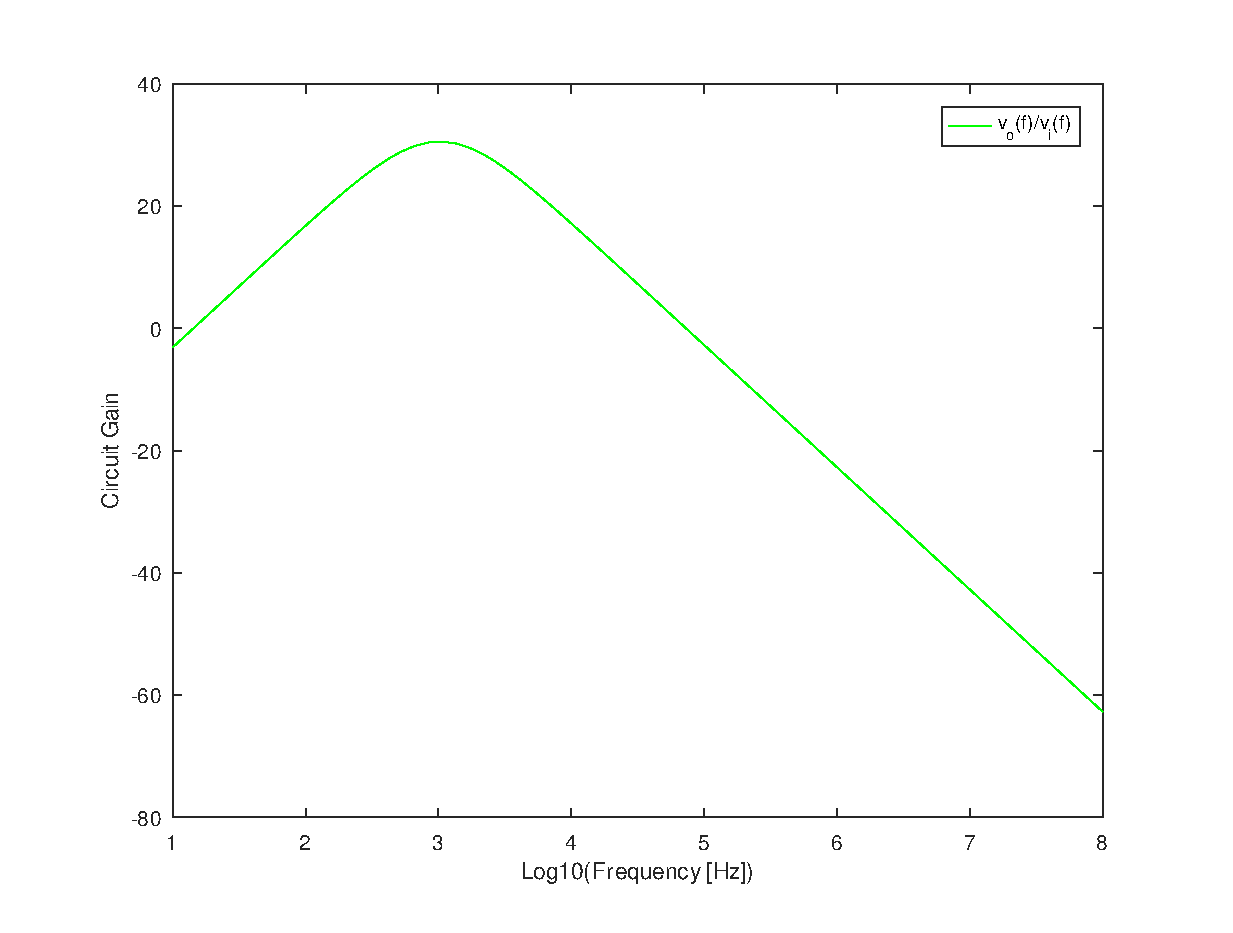
\includegraphics[width=1\linewidth]{teoria.eps}
	\caption{Frequency response of the amplifier ($\frac{V_o(f)}{V_i(f)}$)}
\end{figure}

\par Finally, the theoretical merit is shown below, as well as the high and low cutoff frequencies, the cost and the bandwidth.

\vspace{5mm}
\begin{table}[H]
	\centering
	\begin{tabularx}{0.9\textwidth} {
 	    | >{\raggedright\arraybackslash}X
  	    | >{\raggedleft\arraybackslash}X | }
	\hline
	Merit & 4.921738e+02 \\ \hline
HighCutOff frequency & 4.377991e+05 Hz\\ \hline
LowCutOff frequency & 1.262427e+01 Hz\\ \hline
Cost & 2.198943e+03 MU's\\ \hline
Bandwidth & 4.377865e+05 Hz\\ \hline
Max Gain & 3.111556e+01 V\\ \hline

	\end{tabularx}
	\caption{Theoretical variables of merit}
	\label{tab:merit1}
\end{table}
\vspace{5mm}


\newpage
\section{Simulation}
\label{sec:simulation}

\subsection{First point}
\label{ssec:1S}
\par  With the circuit solved using the mesh and node methods, it's necesssary to solve it experimentally. In order to simulate the real conditions, which we would have encountered in the laboratory, Ngspice was used. The results obtained from this simulation will take in account the energy dissipation due to the many processes that occur such as Joule effect on conductors. Using this software, we were able to verify the results obtained from the methods already described. 

\par  In order to describe the circuit to be studied, it is necessary to follow some guidelines. Firstly, it was needed to specify , for each component, which were its positive and negative nodes. Because of that, the current directions were defined accordingly to the picture shown. As such, the electric resistances, current sources and the capacitor are going to have the positive node in the location of the current input and the negative node in the current output. The voltage sources nodes were defined so that the nodes are in accordance with the pre established nodes.  the picture below, a brief representation of the interpertation of the circuit by the ngspice programme is presented.

\par Apart from this, it was also necessary to establish the values of the resistance, current and voltage associated with the resistors and independent current and voltage sources. The dependent sources, Vc and Ib (Hc and Gb in ngspice because of the symbolic representation in the program), were respectively current controlled voltage source and voltage controlled current source. Because of that, kc and kb were in kOhm and mS as the script indicated. In the case of Vc, it was needed to indicate a control voltage source, Ve which, even though it doesn't exist, is going to measure the current Ic, the control current, passing through it. This voltage control has a null potential so it doesn't interfere with the rest of the circuit. The nodes of Ve were placed in the circuit so that the current input is in the positive node of the voltage source and the output of the current is in the negative node of the source.  In the case of Ib, it was needed to introduce the nodes in which the potential difference is going to be read (again the positive node in first place and then the negative one).

\par The circuit with the considered current directions can be seen in the picture below.

\begin{figure}[h] \centering
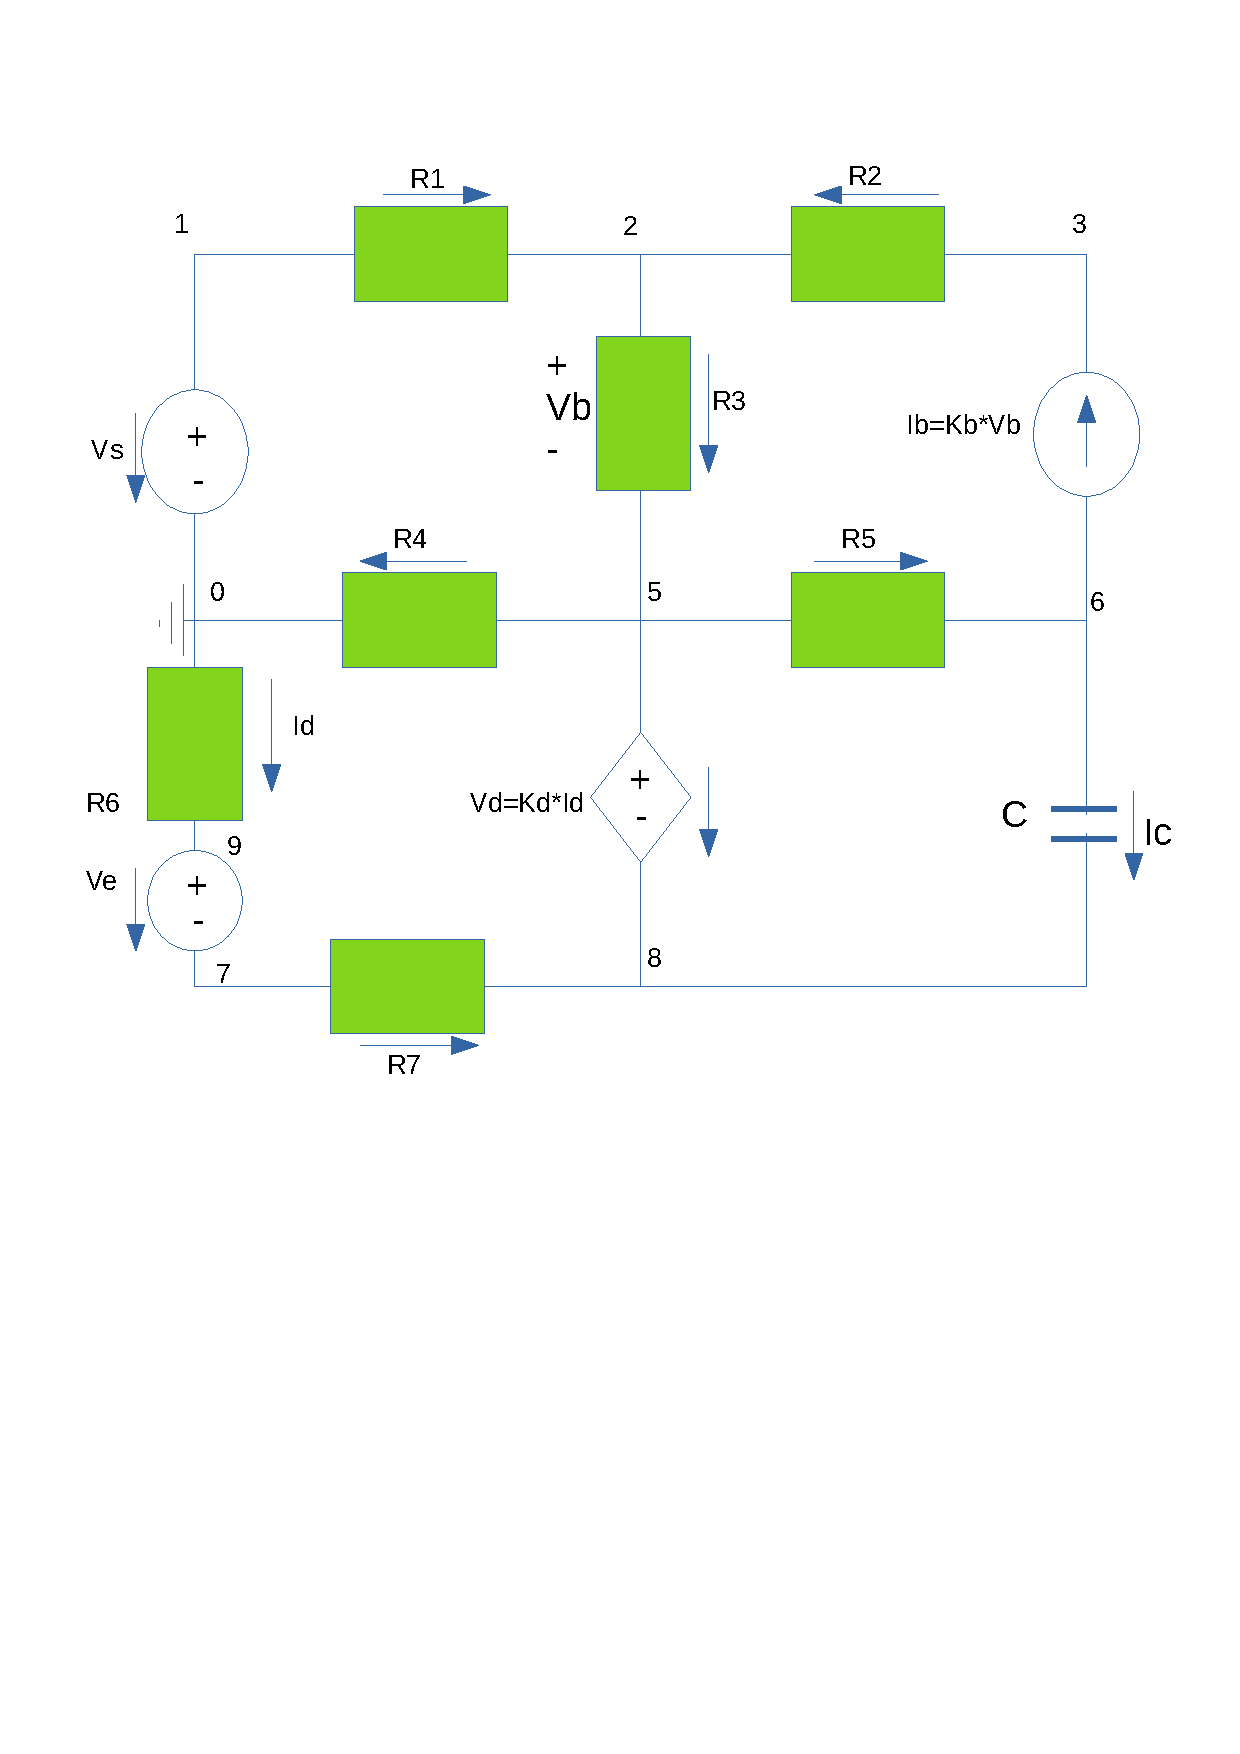
\includegraphics[width=0.6\linewidth]{Desenho_2.pdf}
\caption{Picture of the circuit in analysis with current directions followed in the ngspice simulation}
\label{fig:Ngspice circuit}
\end{figure}

\par For the first point, it is asked to simulate the circuit when t is less than zero. As such, $vs=Vs$ and the current is DC, which means that there is no voltage variation with time in nodes 0 and 1 and, as the other sources are linear, voltage won't varie with time in the nodes. As such, the current which passes through the capacitor is going to be null as there is no variation with the potential difference in it. Runing the simulation (not transient as all intensity and potential values are constant), we obtain a table with the values of the current and voltage in all nodes confirming what was previously said. This confirmes the values calculated through octave in the theoretical analysis. Below a table with the values obtained and the errors associated is shown.

\vspace{5mm}
\begin{table}[H]
\centering
\begin{tabularx}{0.6\textwidth} {
  | >{\raggedright\arraybackslash}X
  | >{\raggedleft\arraybackslash}X | }
 \hline
@ca[i] & 0.000000e+00\\ \hline
@gb[i] & -2.68449e-04\\ \hline
@r1[i] & 2.563813e-04\\ \hline
@r2[i] & -2.68449e-04\\ \hline
@r3[i] & -1.20678e-05\\ \hline
@r4[i] & 1.186012e-03\\ \hline
@r5[i] & -2.68449e-04\\ \hline
@r6[i] & 9.296302e-04\\ \hline
@r7[i] & 9.296302e-04\\ \hline
v(1) & 5.125559e+00\\ \hline
v(2) & 4.861047e+00\\ \hline
v(3) & 4.313554e+00\\ \hline
v(5) & 4.898549e+00\\ \hline
v(6) & 5.710299e+00\\ \hline
v(7) & -1.91255e+00\\ \hline
v(8) & -2.87912e+00\\ \hline
v(9) & -1.91255e+00\\ \hline

\end{tabularx}
\end{table}
\vspace{5mm}

\par Comparing the simulation with the theoretical prediction, we can compute the error associated to each value. The error values are presented in the table bellow.

\vspace{5mm}
\begin{table}[H]
\centering
\begin{tabularx}{0.6\textwidth} {
  | >{\raggedright\arraybackslash}X
  | >{\raggedleft\arraybackslash}X | }
 \hline
@ca[i] & 0.000000e+00 A \\ \hline
@gb[i] & 2.000000e-10 A \\ \hline
@r1[i] & 5.127627e-04 A \\ \hline
@r2[i] & 2.000000e-10 A \\ \hline
@r3[i] & 2.413565e-05 A \\ \hline
@r4[i] & 2.372024e-03 A \\ \hline
@r5[i] & 2.000000e-10 A \\ \hline
@r6[i] & 1.859260e-03 A \\ \hline
@r7[i] & 1.000000e-10 A \\ \hline
v(1) & 0.000000e+00 V \\ \hline
v(2) & 0.000000e+00 V \\ \hline
v(3) & 0.000000e+00 V \\ \hline
v(5) & 0.000000e+00 V \\ \hline
v(6) & 0.000000e+00 V \\ \hline
v(7) & 2.000000e-06 V \\ \hline
v(8) & 6.000000e-06 V \\ \hline
v(9) & 2.000000e-06 V \\ \hline

\end{tabularx}
\end{table}
\vspace{5mm}

\subsection{Second point}
\label{ssec:2S}

\par In this point, the goal is to simulate the operating point for $v_s(0)=0$. In order to accomplish this, we replaced the capacitor with a voltage source $V_x=V(6)-V(8)$, where $V(6)$ and $V(8)$ are the voltages in nodes 6 and 8, respectively, found in point 1. This step is, as explained in subsection \ref{ssec:2T}, based on Thévenin's theorem: we replace the capacitor with $V_s$, then we analyse all node voltages and branch currents; then, knowing $V(6)$, $V(8)$ and $I_x$, we can determine $R_{eq}$ ($R_{eq}=\frac{V_x}{I_x}$), and compute the circuit's time constant ($\tau = R_{eq}C$).
\par The results output by Ngspice are presented in the following table.

\vspace{5mm}
\begin{table}[H]
\centering
\begin{tabularx}{0.6\textwidth} {
  | >{\raggedright\arraybackslash}X
  | >{\raggedleft\arraybackslash}X | }
 \hline
@gb[i] & -1.07836e-18\\ \hline
@r1[i] & 1.029487e-18\\ \hline
@r2[i] & -1.07836e-18\\ \hline
@r3[i] & -4.88721e-20\\ \hline
@r4[i] & -2.21871e-19\\ \hline
@r5[i] & -1.89416e-03\\ \hline
@r6[i] & -2.16840e-19\\ \hline
@r7[i] & -4.26567e-19\\ \hline
v(1) & 0.000000e+00\\ \hline
v(2) & -1.03645e-15\\ \hline
v(3) & -3.22879e-15\\ \hline
v(5) & -8.88178e-16\\ \hline
v(6) & 5.930624e+00\\ \hline
v(7) & 4.540420e-16\\ \hline
v(8) & 8.881784e-16\\ \hline
v(9) & 4.540420e-16\\ \hline

\end{tabularx}
\end{table}
\vspace{5mm}

\par Comparing the simulation with the theoretical prediction, we can compute the error associated to each value. The error values are presented in the table bellow.

\subsection{Third Point}
\label{ssec:3S}

\par In this point, the objective is to simulate the natural response of the circuit in node 6 for $t \in[0;20]$ms, that is, the evolution of this node's voltage throught time, when all independent sources are switched off. As the used boundary condition is $V(6)$ and $V(8)$ equal to the values found in point \ref{ssec:2S} for this nodes, we used the command \textit{.include} in the \textit{Ngspice's} script so that this values are imported automatically.
\par The obtained result is plotted bellow.

\begin{figure}[h] \centering
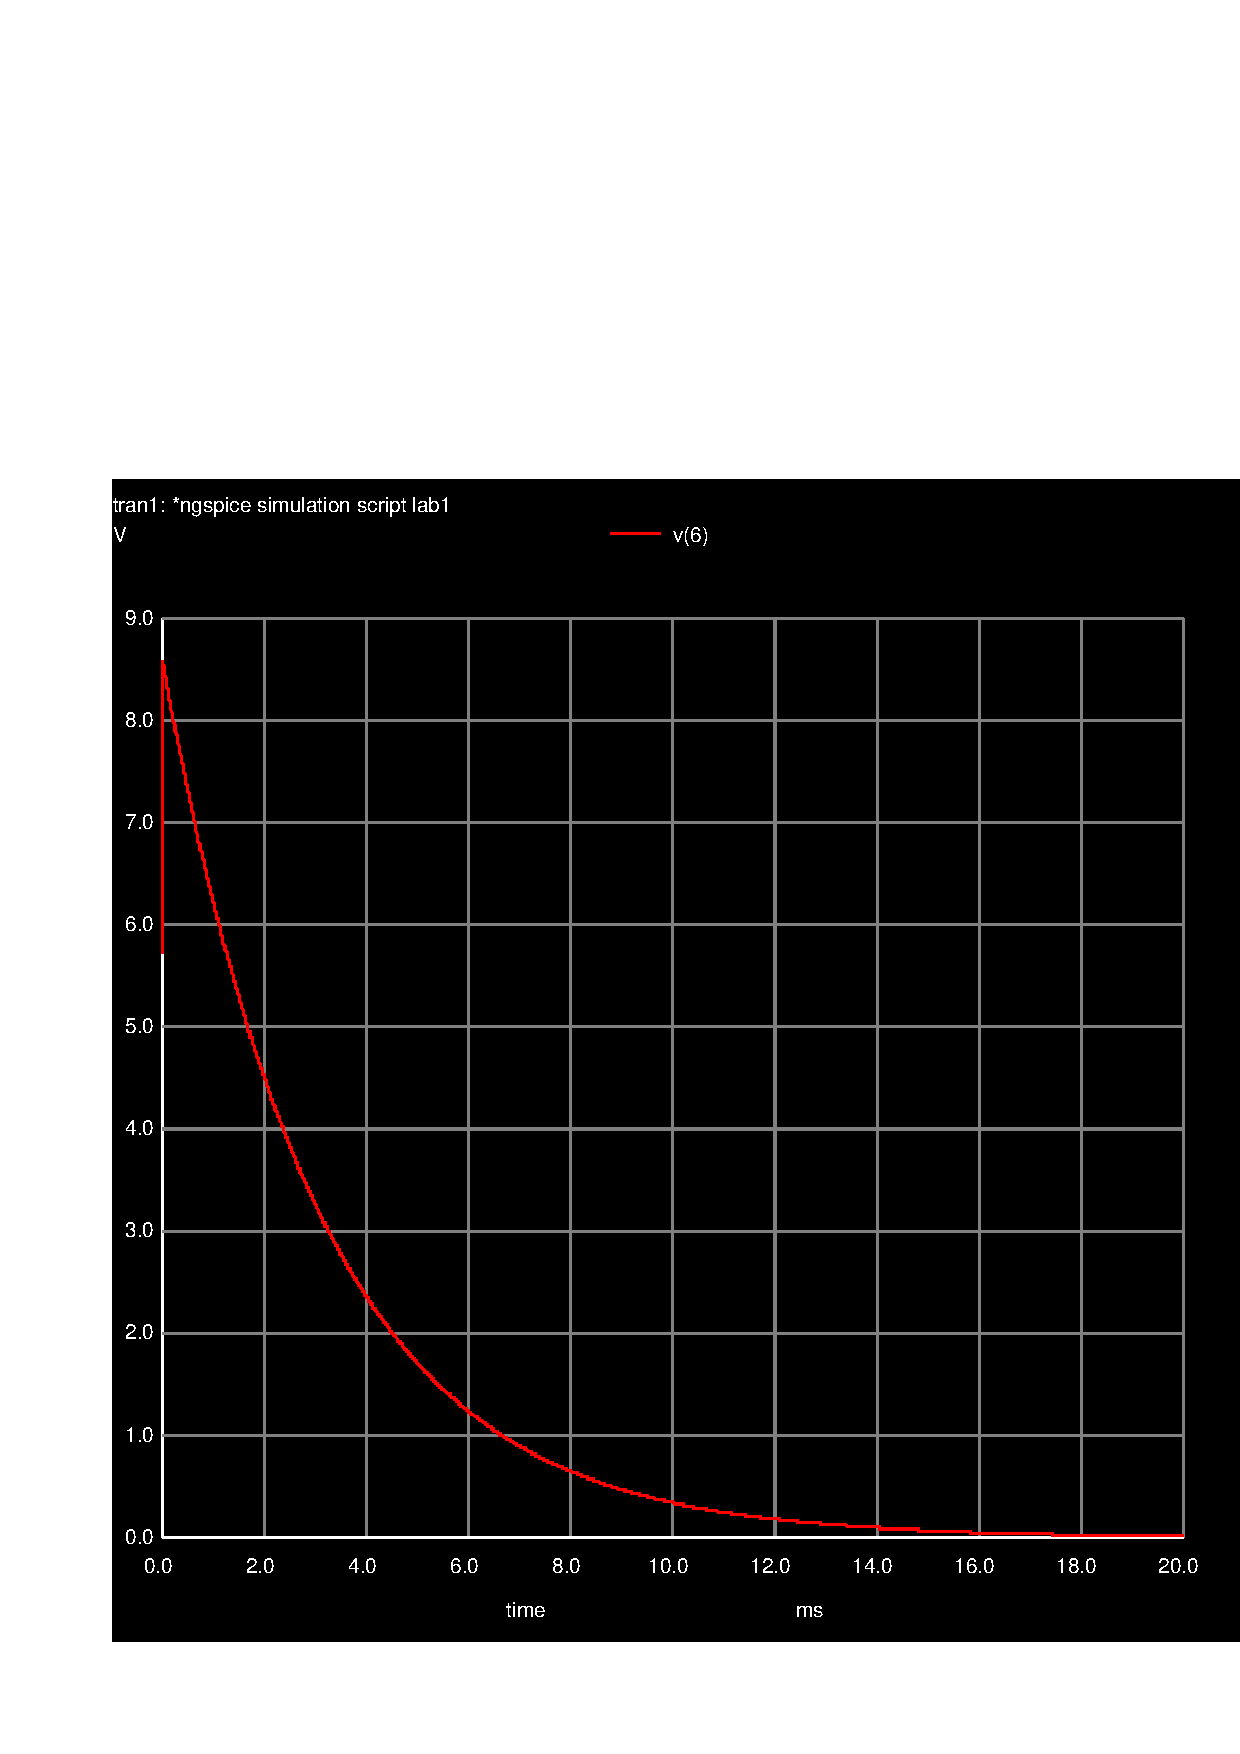
\includegraphics[width=0.7\linewidth]{../sim/teste_3.pdf}
\caption{Natural solution $v_{6n}(t)$, $t\in[0,20]$ms (simulation)}
\label{fig:snat_sim}
\end{figure}


\subsection{Fourth point}
\label{ssec:4S}

\par With the natural response values obtained, it's now asked to simulate the natural and forced response on node 6 now with vs as given in the script. The natural solution, as it doesn't varie with the values of the source in the circuit will be the same in this and the previous case. The forced solution is equivelent to the response of the node when vs is applied to the circuit maintining the condition that initially the values of the voltages in nodes 6 and 8 were the ones calculated in point 2 of the simulation (in order to simplify the code the values used were the ones calculated through octave in question 2). As the values in the nodes at the beggining of the transient simulation aren't the ones in which the circuit is stable, variation of the potential difference through the capacitor is going to happen. This can be seen in the ploted graph in which, v(1) varies around 0V as it is connected to the source and v(6) starts at near 6V and after 20ms is also varying around 0V. Also, as the voltage source response is given by a sinusoidal function, regular variation of the voltage in all the nodes is going to appear as also in them voltage values are given by sinusoidal funtions with the same given frequency (but different amplitudes). As seen in the graph below, regular oscilation can be seen in V(6) and v(1) even though the circuit has stabelized after 20ms.
\par All of this means that, variation of the potential difference through the capacitor is going to be noticeable and current isn't null. Notice that the amplitude of the current source vs is 1 and as seen in the graph amplitude is also 1 in v(1). However, the amplitude of voltage in node 6 is no longer 1 (approx 0.8V) as voltage is loss in the rest of the components of the circuit until the current reaches node 6. 

\begin{figure}[h] \centering
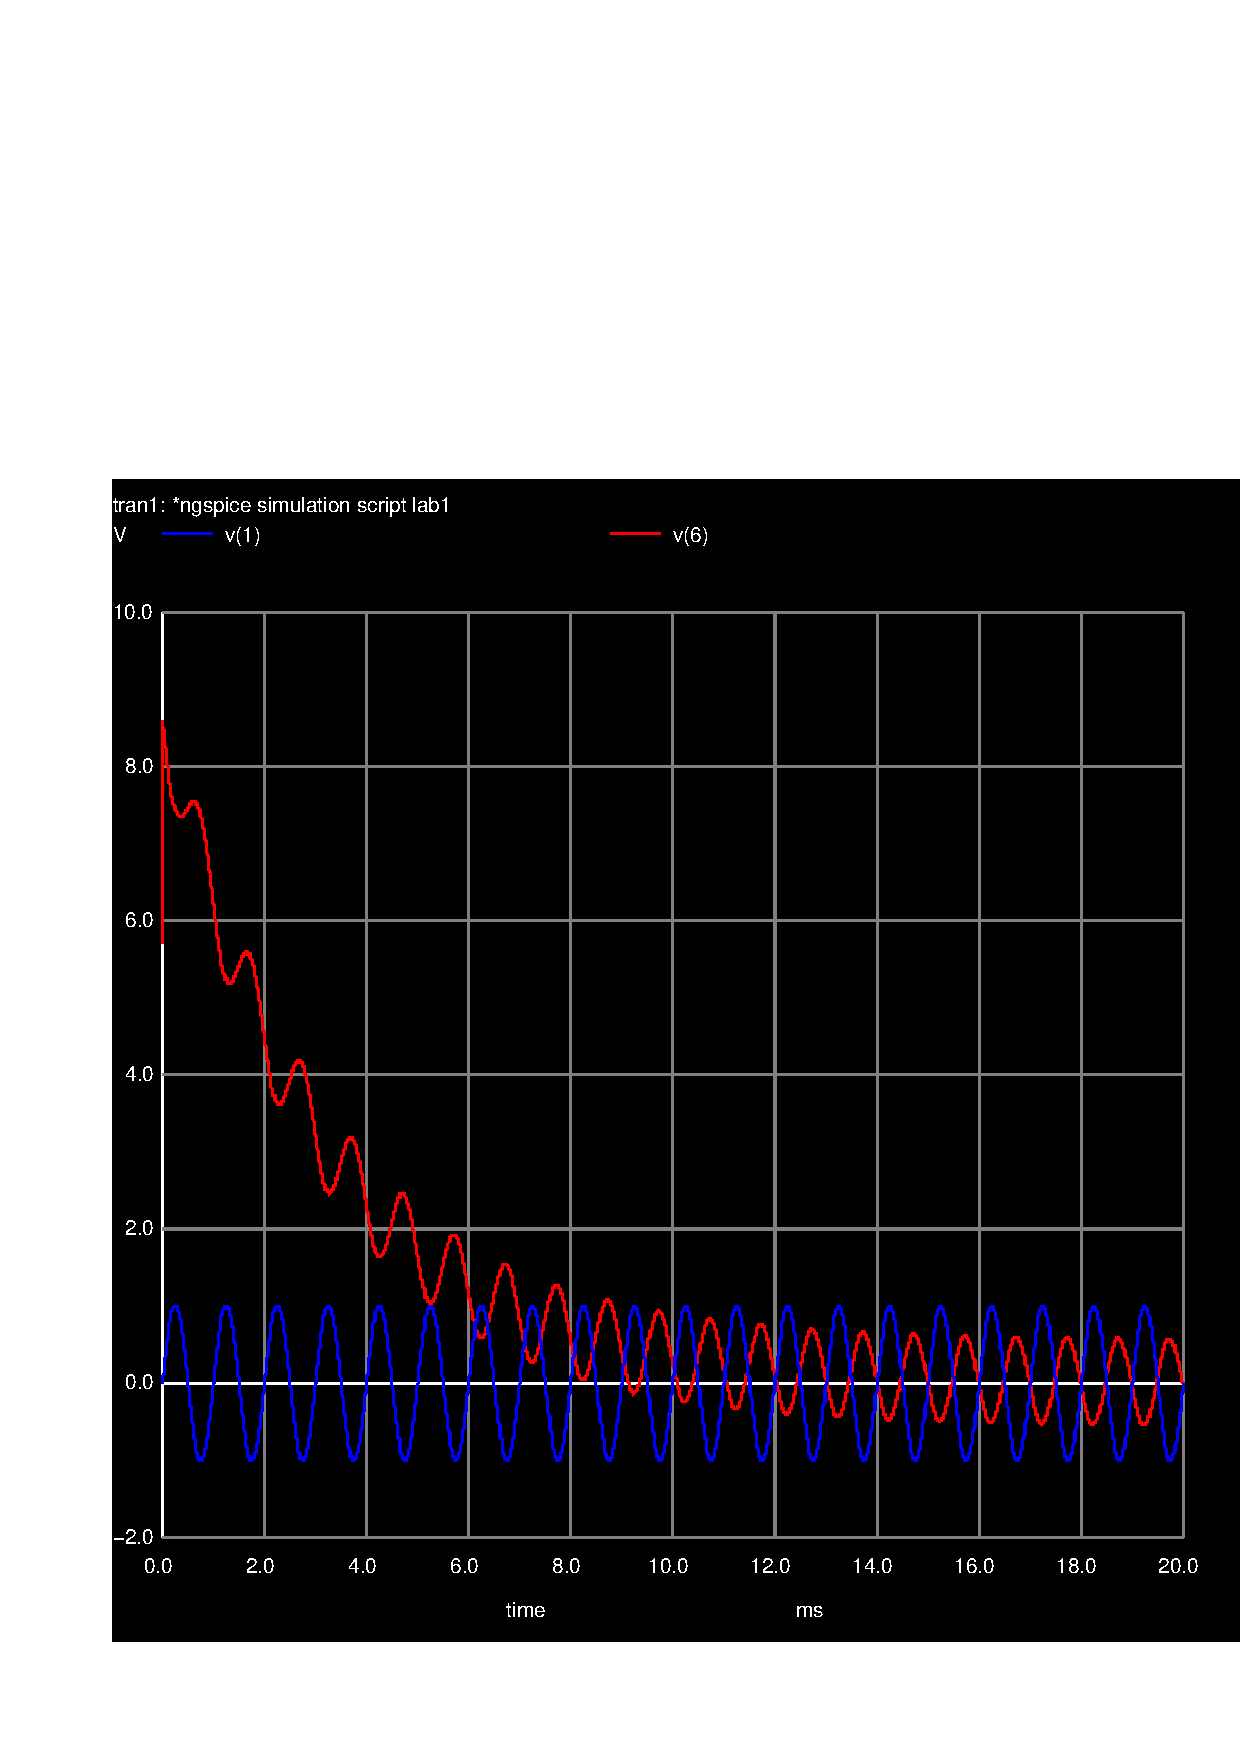
\includegraphics[width=0.6\linewidth]{teste_4.pdf}
\caption{Voltages as functions of time}
\label{fig:V(t)}
\end{figure}

\subsection{Fifth point}
\label{ssec:5S}

\par Finally, in the last question it was studied the frequency response in node 6 through the plot of the phase (rad) in function of the frequency and the magnitude in decibels (in which a 20db increment corresponds to 10x more amplitude) in function of the frequecy of the voltage source and thus the frequecy of the circuit. In these plots a logarithmic scale was used so that the graphics could be read more easily. 

\begin{figure}[h] \centering
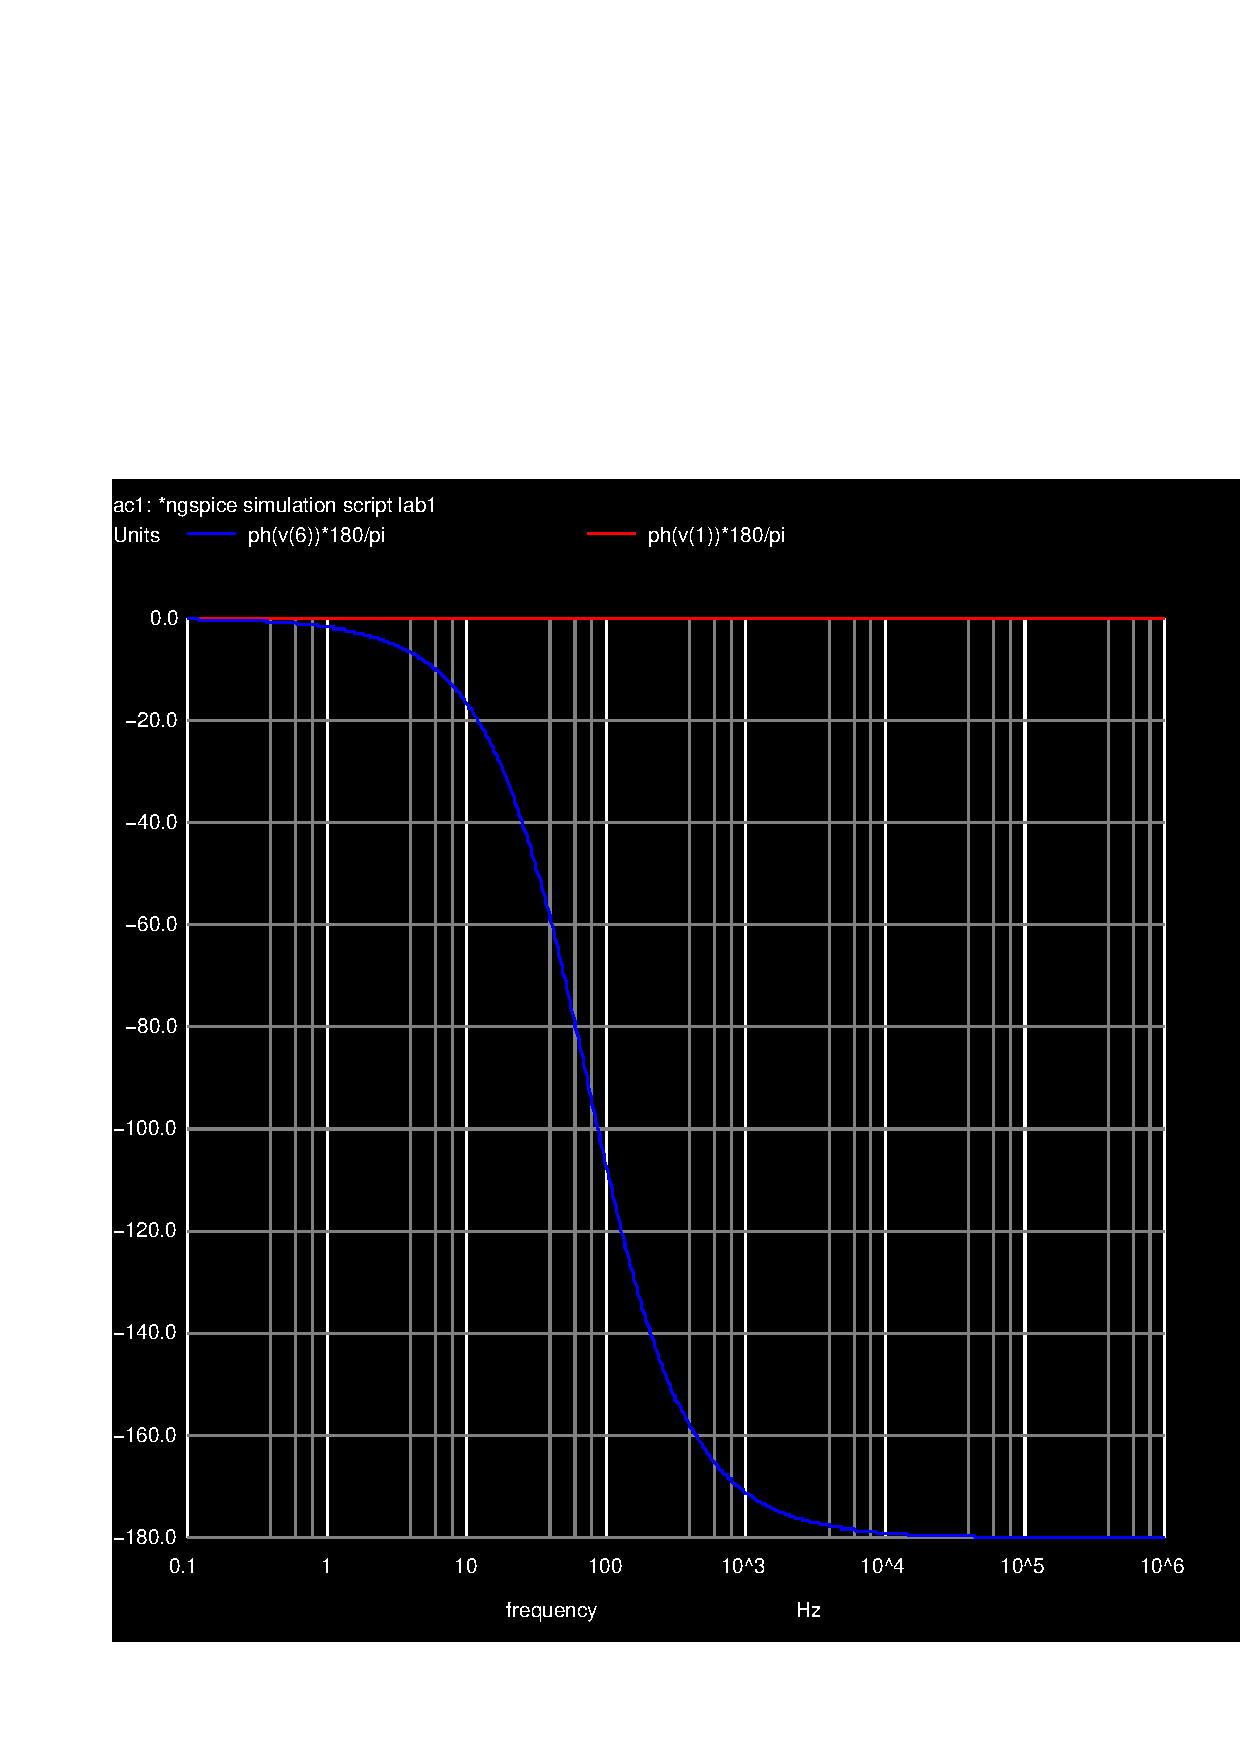
\includegraphics[width=0.6\linewidth]{teste_5_p.pdf}
\caption{Phase as function of frequency}
\label{fig:Ph(v(1))*180/pi Ph(v(6))*180/pi}
\end{figure}

\begin{figure}[h] \centering
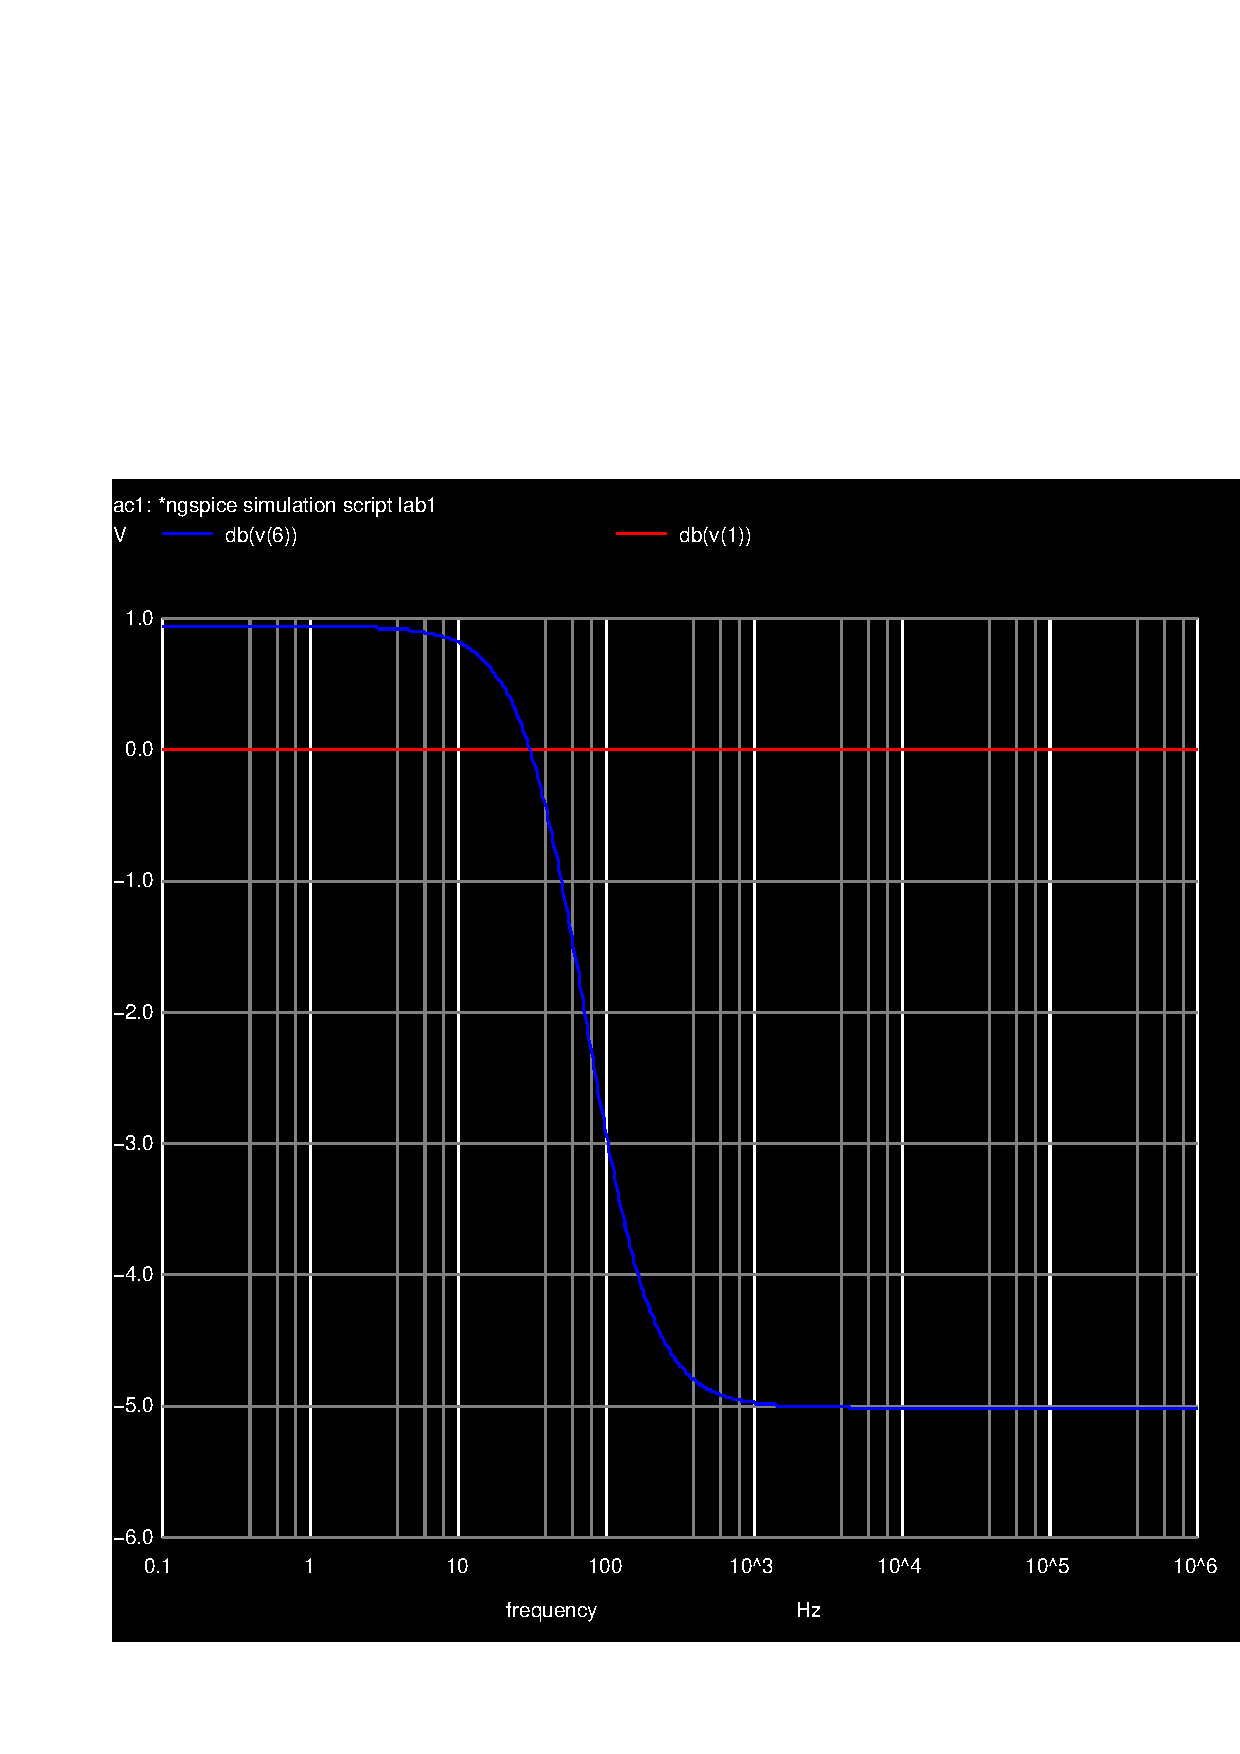
\includegraphics[width=0.6\linewidth]{teste_5_db.pdf}
\caption{Voltage magnitude as function of time}
\label{fig:db(v(1)) db(v(6))}
\end{figure}

\par In the first graphic which describes the phase of v(1) and v(6), as given by the expression intially given of v(1) when $t>0$, its phase is null independently of the value of frequency.  As we can see, the same doesn't happen to the phase of node 6. The reason why this happens can be seen in \ref{ssec:6T}.

\par In the second graphic, the magnitude is expressed in db. In this case, the magnitude of V(1) is constant and null as its magnitude is always 1V and $log(1)=0$. In the case of the magnitude of v(6) as we can see in the equation below, its magnitude varies. The reason why this happens can be seen in \ref{ssec:6T}. 


 

\newpage
\section{Conclusion}
\label{sec:conclusion}

\par In this laboratory assignment, the goal of conceiving an AC/DC converter was achieved. As seen in the whole report, the theoretical results (obtained using Octave) didn't exactly match the simulated ones (obtained using NGspice) because of the non-linearity of the diodes (as predicted), but overall the final result was pretty decent and it's good enough to validate the model used in the theoretical analysis.




%\cleardoublepage

% ----------------------------------------------------------------------
%  Bibliography
% ----------------------------------------------------------------------
%\addcontentsline{toc}{section}{\bibname}
%\bibliographystyle{abbrvunsrtnat} % <<<<< SELECT IF USING REFERENCES BY NUMBER (CITATION ORDER)
%\bibliography{../../../BIBfile.bib}

% ----------------------------------------------------------------------
\end{document}
% ----------------------------------------------------------------------

